% -*- root: paper-esocc.tex -*-

\section{Distributed Monitoring Model}
\label{sec:modelling}

We introduce a distributed monitoring platform and its components and
discuss some underlying assumptions and definitions.
Further, we define the notion of service availability and service budget compliance.
%\begin{wrapfigure}{r}{0.3\textwidth}
%\vspace{-20pt}
%\begin{center}
%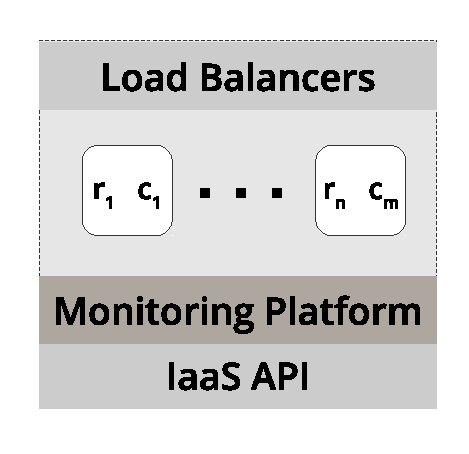
\includegraphics[scale=0.7]{figs/deployment}
%\end{center}
%\vspace{-20pt}
%\caption{{\footnotesize High-level deployment architecture}}
%\label{fig:deployment}
%\vspace{-10pt}
%\end{wrapfigure}
%Figure \ref{fig:deployment} presents a high-level overview of services deployed in a distributed environment (e.g. ``the cloud'').
In the deployment environment (e.g., ``the cloud''), every  server from the IaaS provider is  used for a \emph{single} service of a customer, such as
the Query Service API for a customer of SDL Fredhopper (c.f. Section \ref{sec:fredhopper_example}).
Typically, multiple servers are allocated to a single customer.
The number of servers allocated for a customer is not visible to the customer.
The customer uses a single endpoint - in the load balancer layer - to access all their services.

The ultimate goal is to maintain the environment in such a way that customers and their end users experience the delivered services up to their expectations while minimizing the cost of the system.
%environment does not have a negative impact on the business of SDL Fredhopper.
The first objective can be addressed by adding resources; however, this conflicts with the second goal since it increases the cost of the environment for the customer.
In this section, we formalize the above intuitive notions as \emph{service availability} and \emph{service budget compliance}.

We then develop a distributed monitoring platform that aims to optimize these service
characteristics in a deployment environment.
 % given in Figure \ref{fig:deployment}.
The monitoring platform works in two cyclic phases: \emph{observation} and \emph{reaction}.
The observation phase takes measurements on services in the deployment environment.
Subsequently, the corresponding levels of the service characteristics are calculated.
In the reaction phase, if needed, a platform API is utilized to make the necessary changes to the deployment environment (e.g. adjust the number of allocated resources) to optimize the service characteristics.
% In the monitoring platform, not all components reside in the same resource in the deployment environment; all communications and interactions are performed in an \emph{asynchronous} way.
The monitoring platform builds on top of a real-time extension of the 
actor-based language ABS~\cite{johnsen2012abs}.
To ensure non-intrusiveness of the monitor with the running service,
each monitor is an active object (actor) running on a separate resource
from that which runs the service itself, and the components of the monitoring platform communicate through \emph{asynchronous messages} with deadlines~\cite{johnsen2012modeling}.
% The following elements are the major high-level components of the monitoring platform:
%for a distributed deployment environment: 

Below, we discuss assumptions and basic oncepts that will be used in the
analysis of the formal properties of the monitoring platform and corresponding theorems.
We assume that the external infrastructure provider has an  \emph{unlimited} number of resources.
Further, we assume that all resources are of the \emph{same type}; i.e. they have the same computing power, memory, and IO capacity.
Finally, we assume that every resource   is initialized within  at most $t_i$ amount of time.
%We illustrate and motivate each assumption and definition and discuss how they are generalized from real use-cases from the large deployment environment of the
%SDL Fredhopper cloud.

%\begin{assm}[Unlimited Capacity]
%\label{def:platform:cap}
%We assume that the external infrastructure provider is capable to provision an \emph{unlimited} number of resources.
%\end{assm}

%In reality, every service provider such as SDL Fredhopper has a separate contract with an IaaS provider such as AWS.
%In these contracts, there cannot be a guarantee for \emph{unlimited} capacity.
%We simplify this limitation by assuming that the platform API (IaaS layer abstraction) is capable to provision as many resources as requested.

%\begin{assm}[Single Resource Type]
%\label{def:single:resource:type}
%To simplify reasoning, we assume that all resources are of the \emph{same type}; i.e. they have the same computing power, memory, and IO capacity.
%For example, if we are using AWS,
%we could choose the instance type \jtt{m1.large} for all the services.
%\end{assm}

%If a business delivers different types of services, it cannot avoid the fact that different services may require different \emph{capabilities} from their underlying resources.
%% i.e. one service might require high I/O throughput for its process whereas another might demand high parallelism support from the hardware.
%% Such capability profiles are provisioned through different types of resources from a IaaS provider.
%For example, AWS offers\footnote{\url{http://aws.amazon.com/ec2/instance-types/}} families of EC2 instance types each of which expose different sets of capabilities in terms of computation power, I/O, and network.
%We simplify our analysis by assuming that there is a \emph{single resource type} that is able to provide the necessary capabilities for all services.% in this research scope.

%\begin{assm}[Resource Initialization Time $t_i$]
%\label{def:resource:init:time}
%We assume that every resource $r$ that is initialized is ready for use in at most $t_i$ amount of time.
%% The time $t_i$ is bounded by a finite constant value.
%\end{assm}

%Initialization time can vary between different resource types. The above Assumption \ref{def:single:resource:type} simplifies this: we can just choose the initialization time (a fixed constant) of the single resource type that was chosen.
%The initialization time is also part of the contract with the IaaS provider.
%As discussed above in Assumption \ref{def:single:resource:type}, when a resource is launched and initialized, it might take a different amount of time to be in a state that is \emph{operational} and ready to be used.
%Thus,
%We simplify the property of initialization time of a resource to be a fixed constant for the single resource type that is used in the context of this research.

In our framework
time $T$ is a universally shared clock based on the NTP
\footnote{\url{https://tools.ietf.org/html/rfc1305}} that is used by all elements of the system in the same way. 
$T$ is discrete.
We fix that the unit of time is \emph{milliseconds}.
This level of granularity of time unit means that between
two consecutive milliseconds, the system is not observable.
For example, we use the UTC time standard for all services, monitors and platform API.
We refer to the current time by $t_c$.

We denote by $r$ a resource which provides computational power and storage
and by $s$ a general abstraction of a service in the deployment environment. 
A service exposes an API that is accessible through a delivery layer, such as HTTP.
In our example, a service is the Query API (c.f. Section~\ref{sec:fredhopper_example}) that is accessible through a single HTTP endpoint.

In our framework, 
\emph{monitoring platform}  $P$ is responsible for (de-)allocation of resources for computation or storage.
We abstract from a specific implementation of the monitoring platform $P$ through an API in Listing~\ref{lst:platform}. 
% 
\lstset{language=java,aboveskip=-20pt,belowskip=-20pt}
\begin{wrapfigure}{r}{0.5\textwidth}
% \vspace{-15pt}
\begin{center}
\begin{lstlisting}[mathescape,caption=Platform API,label=lst:platform]
interface Platform {
  void    allocate(Service s);
  void    deallocate(Service s);
  Number  getState(Service s);
  boolean verify$_\alpha$(Service s);
  boolean verify$_\beta$(Service s);
}
\end{lstlisting}
\end{center}   
% \vspace{-15pt}
\end{wrapfigure}
\lstset{mathescape=false}
% 
There is only \emph{one} instance of $P$ available.
In this paper, $P$ internally uses an external infrastructure provisioning API to provide resources (e.g. AWS EC2).
The term ``platform'' is interchangeably used for monitoring in this paper.
The platform provides a method \jtt{getState(Service s)} which returns
the number of resources allocated to the given service $s$ at time $t_c$.

%Monitoring is a runtime analysis approach~\cite{Logean_monitoring}.
We use monitoring to observe the external behavior of a service.
We formalize the external behavior of a service with its service-level agreement (SLA).
An SLA is a contract between the customer (service consumer) and the service provider
which defines (among other things) the minimal quality of the offered service,
and the compensation if this minimal level is not reached.
To formally analyze an SLA, we introduce the notion of a service metric function.
We make basic measurements of the service externally in a given monitoring window (a duration).
The service metric function aggregates the basic measurements into a single number
that indicates the quality of a certain service characteristic (higher numbers are better).
%
%monitoring window measurement.
%The quantified measurements projected to a monitoring window lead to an understanding of the quality of the service based on its SLA.

\emph{Basic measurement} $\mu(s,r,t)$ is a function that produces a real number of a \emph{single} monitoring check on a resource $r$ allocated to service $s$ at some time $t$.  
For example, for SDL Fredhopper cloud services, a basic measurement is the number of completed queries at the current time. 
% 

\emph{Service Metric} $f_s$ is a function that aggregates a sequence of basic non-negative measurements to a single non-negative real value:
$f_s : \bigcup_n \mathbb{R}^n \rightarrow \mathbb{R}$.
For example, for SDL Fredhopper cloud services, the service metric function
$f_s$ calculates the average number of queries per second (\qps) given a list of basic measurements.

\emph{Monitoring Window} is a duration of time $\tau$ throughout which basic measurements for a service are taken.
% 

\emph{Monitoring Measurement} is a function that aggregates the basic measurements for a service over its resources in the last monitoring window.
The last monitoring window is defined as $[t_c-\tau, t_c]$.
To produce the monitoring measurement, $f_s$ is applied.
Formally:
\[
\mu(s,r,\tau) = 
f_s \big(\langle \mu_i(s,r,t) \rangle^{\infty}_{i=0}\big) \;\; \textnormal{where} \;\; t \in [t_c-\tau, t_c] 
\]
in which $\mu_i(s,r,t)$ is the $i$-th basic measurement of services $s$ on resource $r$ at time $t$ where $t \in [t_c-\tau,t_c]$.


\begin{defn}[Service Availability $\alpha(s,\tau,t_c)$]
\label{def:service:availability}
% 
First, we need a few auxiliary definitions before we can define service availability.
% 


\emph{Service Capacity} $\kappa_\sigma(s,\tau) = \sum_{r \in \sigma(s)} \mu(s,r,\tau)$ denotes the  capability of service $s$ that is the aggregated monitoring measurements of its resources over the monitoring window $\tau$ and $\sigma(s)$ is the number of allocated resources to service $s$.
% 

\emph{Agreement Expectation} $E(s,\tau, t_c)$ is the minimum number of requests that a customer expects to complete in a monitoring window $\tau$.
The agreement expectation depends on the current time $t_c$ because the expectation may change over time.
For example, SDL Fredhopper customers expect a different \qps during Christmas.
% 

We define the availability of a service $\alpha(s,\tau,t_c)$ in every monitoring window $\tau$ as:
% \vspace{-10pt}
\[
\alpha(s,\tau,t_c) = \frac{\kappa_\sigma(s,\tau)}{E(s,\tau,t_c)}
\]
% in every monitoring window $\tau$.
% 

\emph{Capacity Tolerance} $\varepsilon_\alpha(s,\tau)) \in [0,1]$ defines how much $\kappa_\sigma(s,\tau)$ can deviate from $E(s,\tau,t_c)$ in every time span
of duration $\tau$.
\end{defn}
% 

\emph{Service Guarantee Time $t_G$} is the duration within which a customer expects service availability reaches an acceptable value after a violation. 
Typically, $t_G$ is an input parameter from the customer's contract.


\begin{exmp}
Intuitively, $\alpha(s,\tau,t_c)$ presents the actual capability of a service $s$ over a time period $\tau$ compared to the expectation on the service $E(s,\tau)$. 
For values $\alpha(s,\tau,t_c) \ll 1 - \varepsilon_\alpha(s,\tau))$, the resource for service $s$ are at ``under-capacity'' while for values $\alpha(s,\tau,t_c) \gg 1 + \varepsilon_\alpha(s,\tau))$, there is ``over-capacity''. The goal is optimize $\alpha(s,\tau,t_c)$ towards a value of 1.
% 

For example, we expect a query service to be able to complete 10 queries per second. 
We define the monitoring window $\tau = $ 5 minutes; thus, $E(s,\tau,t_c) = 10 \times 60 \times 5 = 3000$.
Suppose we allocate only one resource to the service,
measure the service during a single monitoring window $\tau$
and find $\mu(s,r,\tau) = 2900$. Then $\alpha(s,\tau,t_c) = \frac{2900}{3000} = 0.966$.
If we have $\varepsilon_\alpha(s,\tau)) = 0.03$, this means that service $s$ is under-capacity because $\alpha(s,\tau,t_c) < 1 - \varepsilon_\alpha$.
\end{exmp}

\begin{defn}[Budget Compliance $\beta(s,\tau)$]
\label{def:budget:compliance}
% 
We first provide a few auxiliary definitions.
% 

\emph{Resource Cost} $\euro(r,\tau) \in \mathbb{R}^+$ is the cost of resource $r$ in a monitoring window $\tau$ which is determined by a fixed resource cost per time unit.

\emph{Service Cost} $\euro_\sigma(s,\tau) \in \mathbb{R}^+$ is the cost of a service $s$ in a monitoring window $\tau$ and defined as $\euro_\sigma(s,\tau) = \sum_{r \in \sigma(s)} \euro(r,\tau)$.
% 

\emph{Service Budget} $B(s,\tau)$ specifies an upper bound of the expected cost of a service in the time span $\tau$.
Intuitively $B(s,\tau)$ is the allowed budget that can be spent for service $s$ over the time span $\tau$.
%Note that
The service budget is typically chosen to be fixed over any time span $\tau$.
% 

We are now ready to define service budget compliance $\beta(s,\tau)$ that,
intuitively, represents how a service complies with its allocated budget:
\[
\beta(s,\tau) = \frac{\euro_\sigma(s,\tau)}{B(s,\tau)}
\]

\emph{Budget Tolerance} $\varepsilon_\beta(s,\tau) \in [0,1]$ specifies how much the service cost $\euro(s,\tau)$ can deviate from $B(s,\tau)$ in every time span of duration $\tau$.

\emph{Service Guarantee Time} $t_G$ is similar to that defined for service availability.
% 
\end{defn} % end - budget compliance

\begin{exmp}
% during its runtime. 
Assume every resource on the environment costs $1$ (e.g. $\euro$) per hour.
Suppose we set a budget of $1.5$ per hour for every service,
allocate \emph{one} resource to the service and define a monitoring window of $\tau = 5$ minutes.
Every hour has $12$ monitoring windows.
This means that each resource costs $\euro(r,\tau) = \frac{1}{12} \approx 0.08$ per monitoring window.
Since there is only one resource, the service cost is $\euro(s,\tau) = \sum_{r\in\sigma(s)}\euro(s,\tau) \approx 0.08$ per monitoring window.
On the other hand, if we calculate the budget for one monitoring window, we have $B(s,\tau) = \frac{1.5}{12} = 0.125$ per monitoring window.
This yields budget compliance as $\beta(s,\tau) = \frac{0.08}{0.125} = 0.64$.
\end{exmp}
% 

% The formal definitions above provide a basis
% to react appropriately to changes or failures in an environment.
% We enumerate a few as follows.
% 
% A service $s$ is ``under-capacity'' as long as $\alpha(s,\tau,t_c) < 1 - \varepsilon_\alpha(s,\tau))$; 
% i.e. intuitively this means that the service cannot provide the expected quality to
% end-users.
% To fix an under-capacity service, \emph{new} resources through the monitoring platform $P$ can be requested (scale up) to increase the capacity of $s$.
% Similarly, service $s$ can be ``over-capacity'';
% i.e. $\alpha(s,\tau,t_c) \gg 1 + \varepsilon_\alpha(s,\tau))$.
% An important disadvantage of an over-capacity service is that it \emph{costs} more than necessary to deliver what is expected from it.
% To improve an over-capacity service, at least one of the current resources allocated to service $s$ can be terminated (scale down) as long as this does not result in an ``under-capacity'' service.
%Similarly, a service can be ``over-budget'' and ``under-budget'', and corresponding actions can be taken to resolve that.

The formal definitions of service availability and budget compliance provide a rigorous 
basis for automatic deployment of resource-aware services with an appropriate quality of service, taking costs into account.
%Properties $\alpha(s,\tau,t_c)$ and $\beta(s,\tau)$ of a service $s$ build a foundation facilitate \emph{automation of operation} of the service according to its properties. 
This in particular includes automated scaling up or down of the service with the help of monitoring checks that are installed for the service. 
%However,
The fundamental challenge in ensuring service availability and budget compliance is that they have \emph{conflicting} objectives:
\[
\alpha(s,\tau,t_c) \uparrow \iff \beta(s,\tau) \downarrow
\]
Intuitively, if more resources are used to ensure the availability of a service; then $\alpha(s,\tau,t_c)$ increases.
However, at the same time, the service costs more; i.e. budget compliance $\beta(s,\tau)$ decreases.

% In the following sections, we first present two separate timed automata~\cite{alur:1994:timedautomata} to model the behavior of $\alpha(s,\tau,t_c)$ and $\beta(s,\tau)$.
% Then, we formalize how the two can be composed to form a new property called service sustainability $\gamma(s,\tau)$.

% In the next section, we design a timed automata for each service characteristics.
% We show how the timed automata can be used to evolve the systems towards SLA optimizations.
% We present a generalization of the characteristics and how they can be composed together.
